%\chapter{Výsledky práce}

\chapter{Návrh aplikace}
\section{Architektura aplikace}

Aplikace běžící na Raspberry Pi je napsána v programovacím jazyce Python verze 3.5. Aplikace se spustí po startu operačního systému a provede inicializaci vlákna pro stahování konfiguračního souboru v daných intervalech, poté provede inicializací vlákna pro upload fotografií.

\subsection*{Vícevláknové zpracování}
Aplikace bude provádět současně několik činností.

Bude nutné nepřetržitě monitorovat pohyb, odesílat fotografie a současně vyčítat stav baterie. Také je důležité kontrolovat, zda nedošlo ke změně konfigurace. Z toho důvodu bude třeba program rozdělit do více na sobě nezávislých vláken.

\begin{figure}[h]
  \begin{center}
    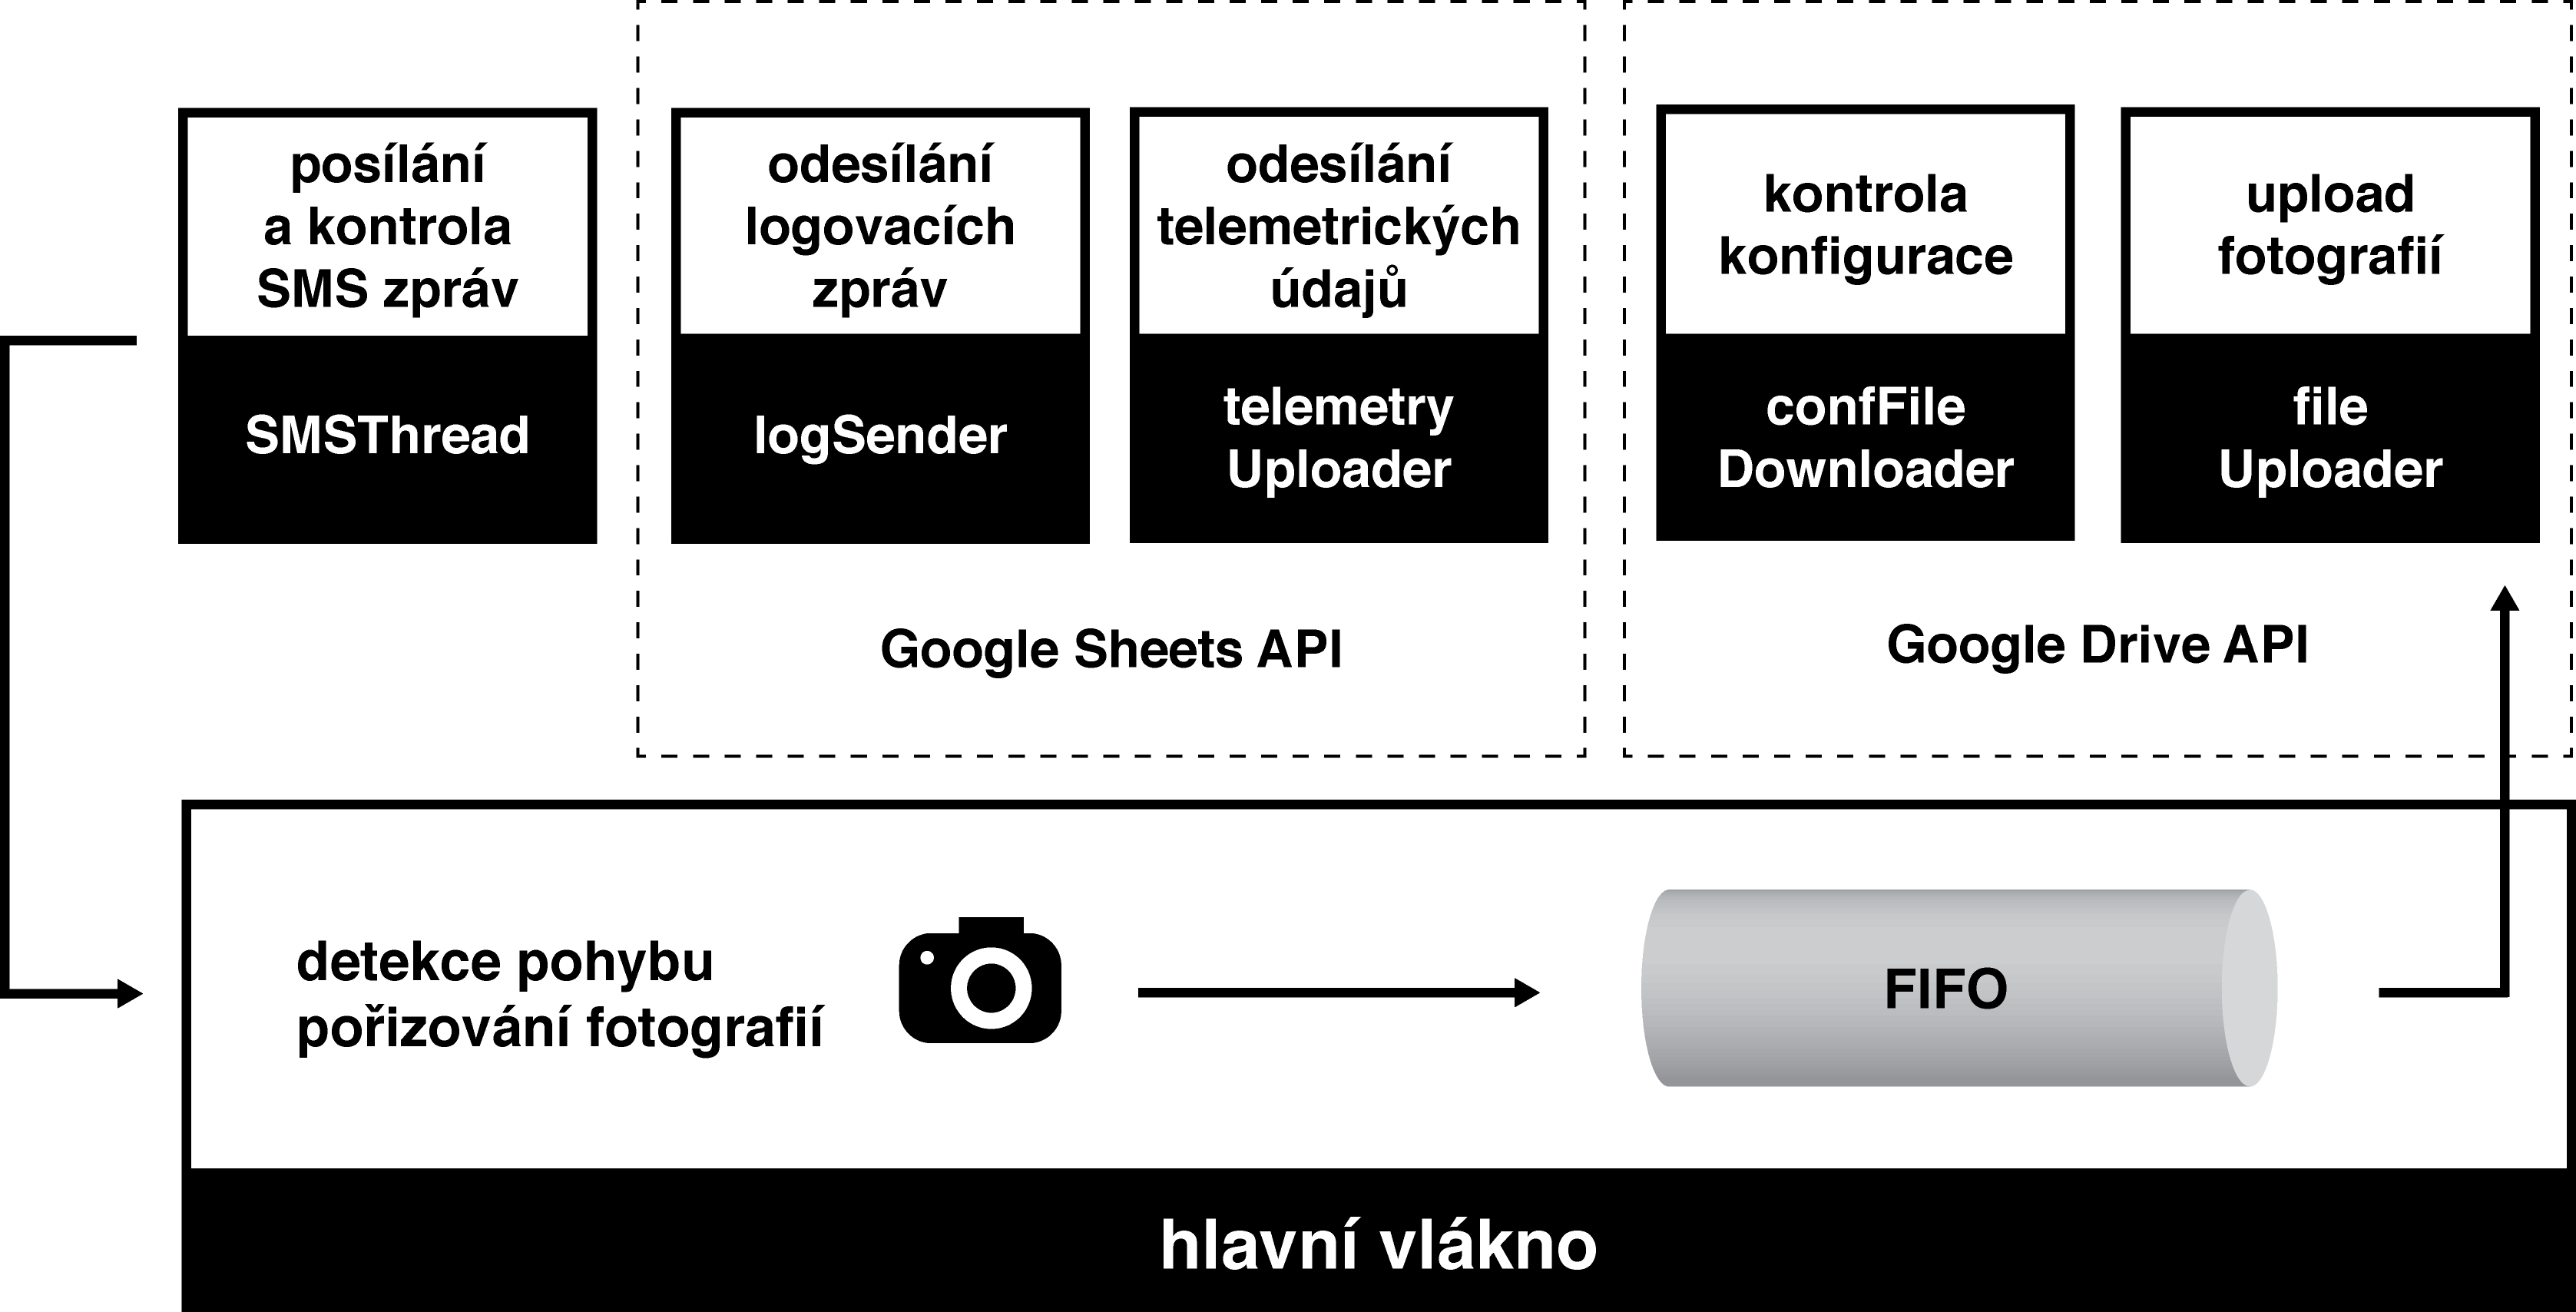
\includegraphics[scale=0.5]{obrazky/schema_aplikace.png}
  \end{center}
  \caption{Architektura aplikace}
\end{figure}

\subsection*{Hlavní vlákno aplikace}
Hlavní vlákno aplikace se stará o detekci pohybu a pořizování fotografií.

Jakmile je detekován pohyb, je provedena zkušební fotografie, ze které je odečtena celková jasová složka snímaného obrazu.

Pokud je hodnota jasu pod prahem denního snímání, jsou nastaveny parametry kamery pro noční režim a je pořízena fotografie.

 Fotografie je zkomprimována, uložena na SD kartu a vložena do fronty pro zaslání do externího úložiště.
 
 Pokud je aktivovaný režim echo, je provedeno ještě dalších 10 fotografií v sekundových intervalech.

\subsection*{Odesílání fotografií do úložiště}
Odesílání fotografií je řešeno ve vlákně nazvaném fileUploader.

Toto vlákno umožňuje autentizaci s Google Drive pomocí OAuth 2.0. Následně je vyčítána fronta a fotografie jsou postupně odesílány do úložiště.

Pokud je aplikace v režimu batch, je odesílání fotografií aktivováno až ve stanovenou dobu.

\subsection*{Kontrola konfigurace}
Vlákno kontroly a stahování konfiguračního souboru zvané confFileDownloader rovněž používá Google Drive API.

Po spuštění vlákna se inicializuje spojení s Google Drive a stáhne se JSON konfigurační soubor podle zadaného identifikátoru. JSON data v konfiguračním souboru jsou přečtena pomocí modulu JSON a naimportována do třídy UserConfig.

V rámci aplikace jsou konfigurační data uložena v modulu config ve třídách BaseConfig a UserConfig, přičemž třídu BaseConfig nelze konfigurovat pomocí JSON a třída UserConfig je určena pro uživatelskou konfiguraci.

Stahování konfiguračního souboru a kontrola změny probíhá ve stanovených intervalech, výchozí hodnota je každých 5 sekund. Pokud vlákno nepracuje, je uspáno.

\subsection*{Odesílání telemetrických údajů}
Vlákno odesílání telemetrických údajů využívá Google Sheets API ke komunikaci s Google Sheets.

Vlákno vyčítá informace o stavu nabíjení akumulátoru ze solárního regulátoru a také informace o využití systémových prostředků jako vytížení CPU a využití operační paměti.

Data se převádí do podoby, kterou je možné vložit do tabulky Google Sheets. Vyčítání dat a odesílání do tabulky je prováděno každých 5 sekund.

\subsection*{Odesílání logovacích zpráv}
Vlákno odesílání logovacích zpráv využívá Google Sheets API ke komunikaci s Google Sheets. 

Vlákno je implementováno jako takzvaný handler pro modul logging, který je využíván pro logování zpráv. Namísto ukládání logovacích zpráv do souboru se zprávy ukládají do fronty a v daných intervalech jsou poslány do listu Google Sheets. 

\subsection*{Odesílání a kontrola SMS zpráv}
Vlákno SMSThread provádí kontrolu přijatých zpráv.

Pokud je přijata SMS zpráva s významem z autorizovaného čísla, tak se provede akce. Pokud je přijata zpráva z neautorizovaného čísla, tak je okamžitě vymazána.

\section{Detekce pohybu}

Zařízení umožňuje dvě metody detekce pohybu - detekce pohybu z obrazu a detekce pohybu pomocí PIR čidla.

Ve výchozím nastavení jsou zapnuty obě metody detekce, avšak detekci pohybu pomocí PIR senzoru je možné vypnout.  

Detekční úhel je dán omezením horizontálního pozorovacího úhlu zvolené kamery. V našem případě výrobce kamery udává pozorovací úhel 62 úhlových stupňů v horizontálním směru a 48 úhlových stupňů ve vertikálním směru.

\subsection*{Detekce pohybu pomocí PIR}
Výhodou detekce pohybu pomocí PIR senzoru je nezávislost na osvětlení scény. Je možné ji použít například v noci, kdy již nelze použít detekci pohybu z obrazu z důvodu necitlivosti kamery.

Další výhodou detekce pohybu PIR senzorem je nízká výpočetní náročnost, protože je kontrolována pouze jedna logická hodnota. 

Efektivita detekce pohybu PIR senzorem je dána těmito parametry: citlivosti PIR senzoru, pozorovacím úhlem kamery a dosahem LED přísvitu.

PIR senzor použitý v této práci má udávanou spolehlivou detekční vzdálenost maximálně 5 metrů, z čehož vyplývá dosah LED přísvitu, tedy také 5 metrů.

\subsection*{Detekce pohybu z obrazu}
Výhodou detekce pohybu z obrazu je kupříkladu možnost umístit kameru za sklo, respektive okno. V případě detekce pohybu pomocí PIR senzoru toto není možné.

Detekce pohybu z obrazu využívá algoritmus výpočtu vektorů pohybu z optického toku.

Tato softwarová metoda je výpočetně velmi náročná, ale patří mezi nejspolehlivější metody. Není tolik ovlivňována změnou osvětlení na snímané scéně a je odolná proti šumu.

V případě Raspberry Pi je kodér H.264 implementován přímo na GPU. Tento princip se využívá například v kodéru MPEG pro kompresi videa.

\subsection*{Hledání vektorů pohybu}
Data o vektorech pohybu je možné získat přímo z kodéru H.264.

V našem případě snímáme video v rozlišením 640x368 pixelů. Vektory pohybu jsou počítány přímo na úrovni makrobloků (makroblok má rozměry 16x16 pixelů).

V našem případě bude tedy mít matice vektorů pohybu rozměry 40+1 sloupců a 23 řádků. Matice obsahuje jeden sloupec dat navíc.

Data o pohybu mají velikost 4 bajty. Každá z proměnných vektoru pohybu [x] a [y] má velikost jeden bajt, zbývající dva bajty obsahují sumu absolutních diferencí (SAD). 

Suma absolutních diferencí udává míru odlišnosti mezi referenčním blokem a současným blokem. Je vypočtena jako suma rozdílů absolutních hodnot mezi jednotlivými pixely v původním bloku a bloku, který porovnáváme. 

\begin{figure}[h]
  \begin{center}
    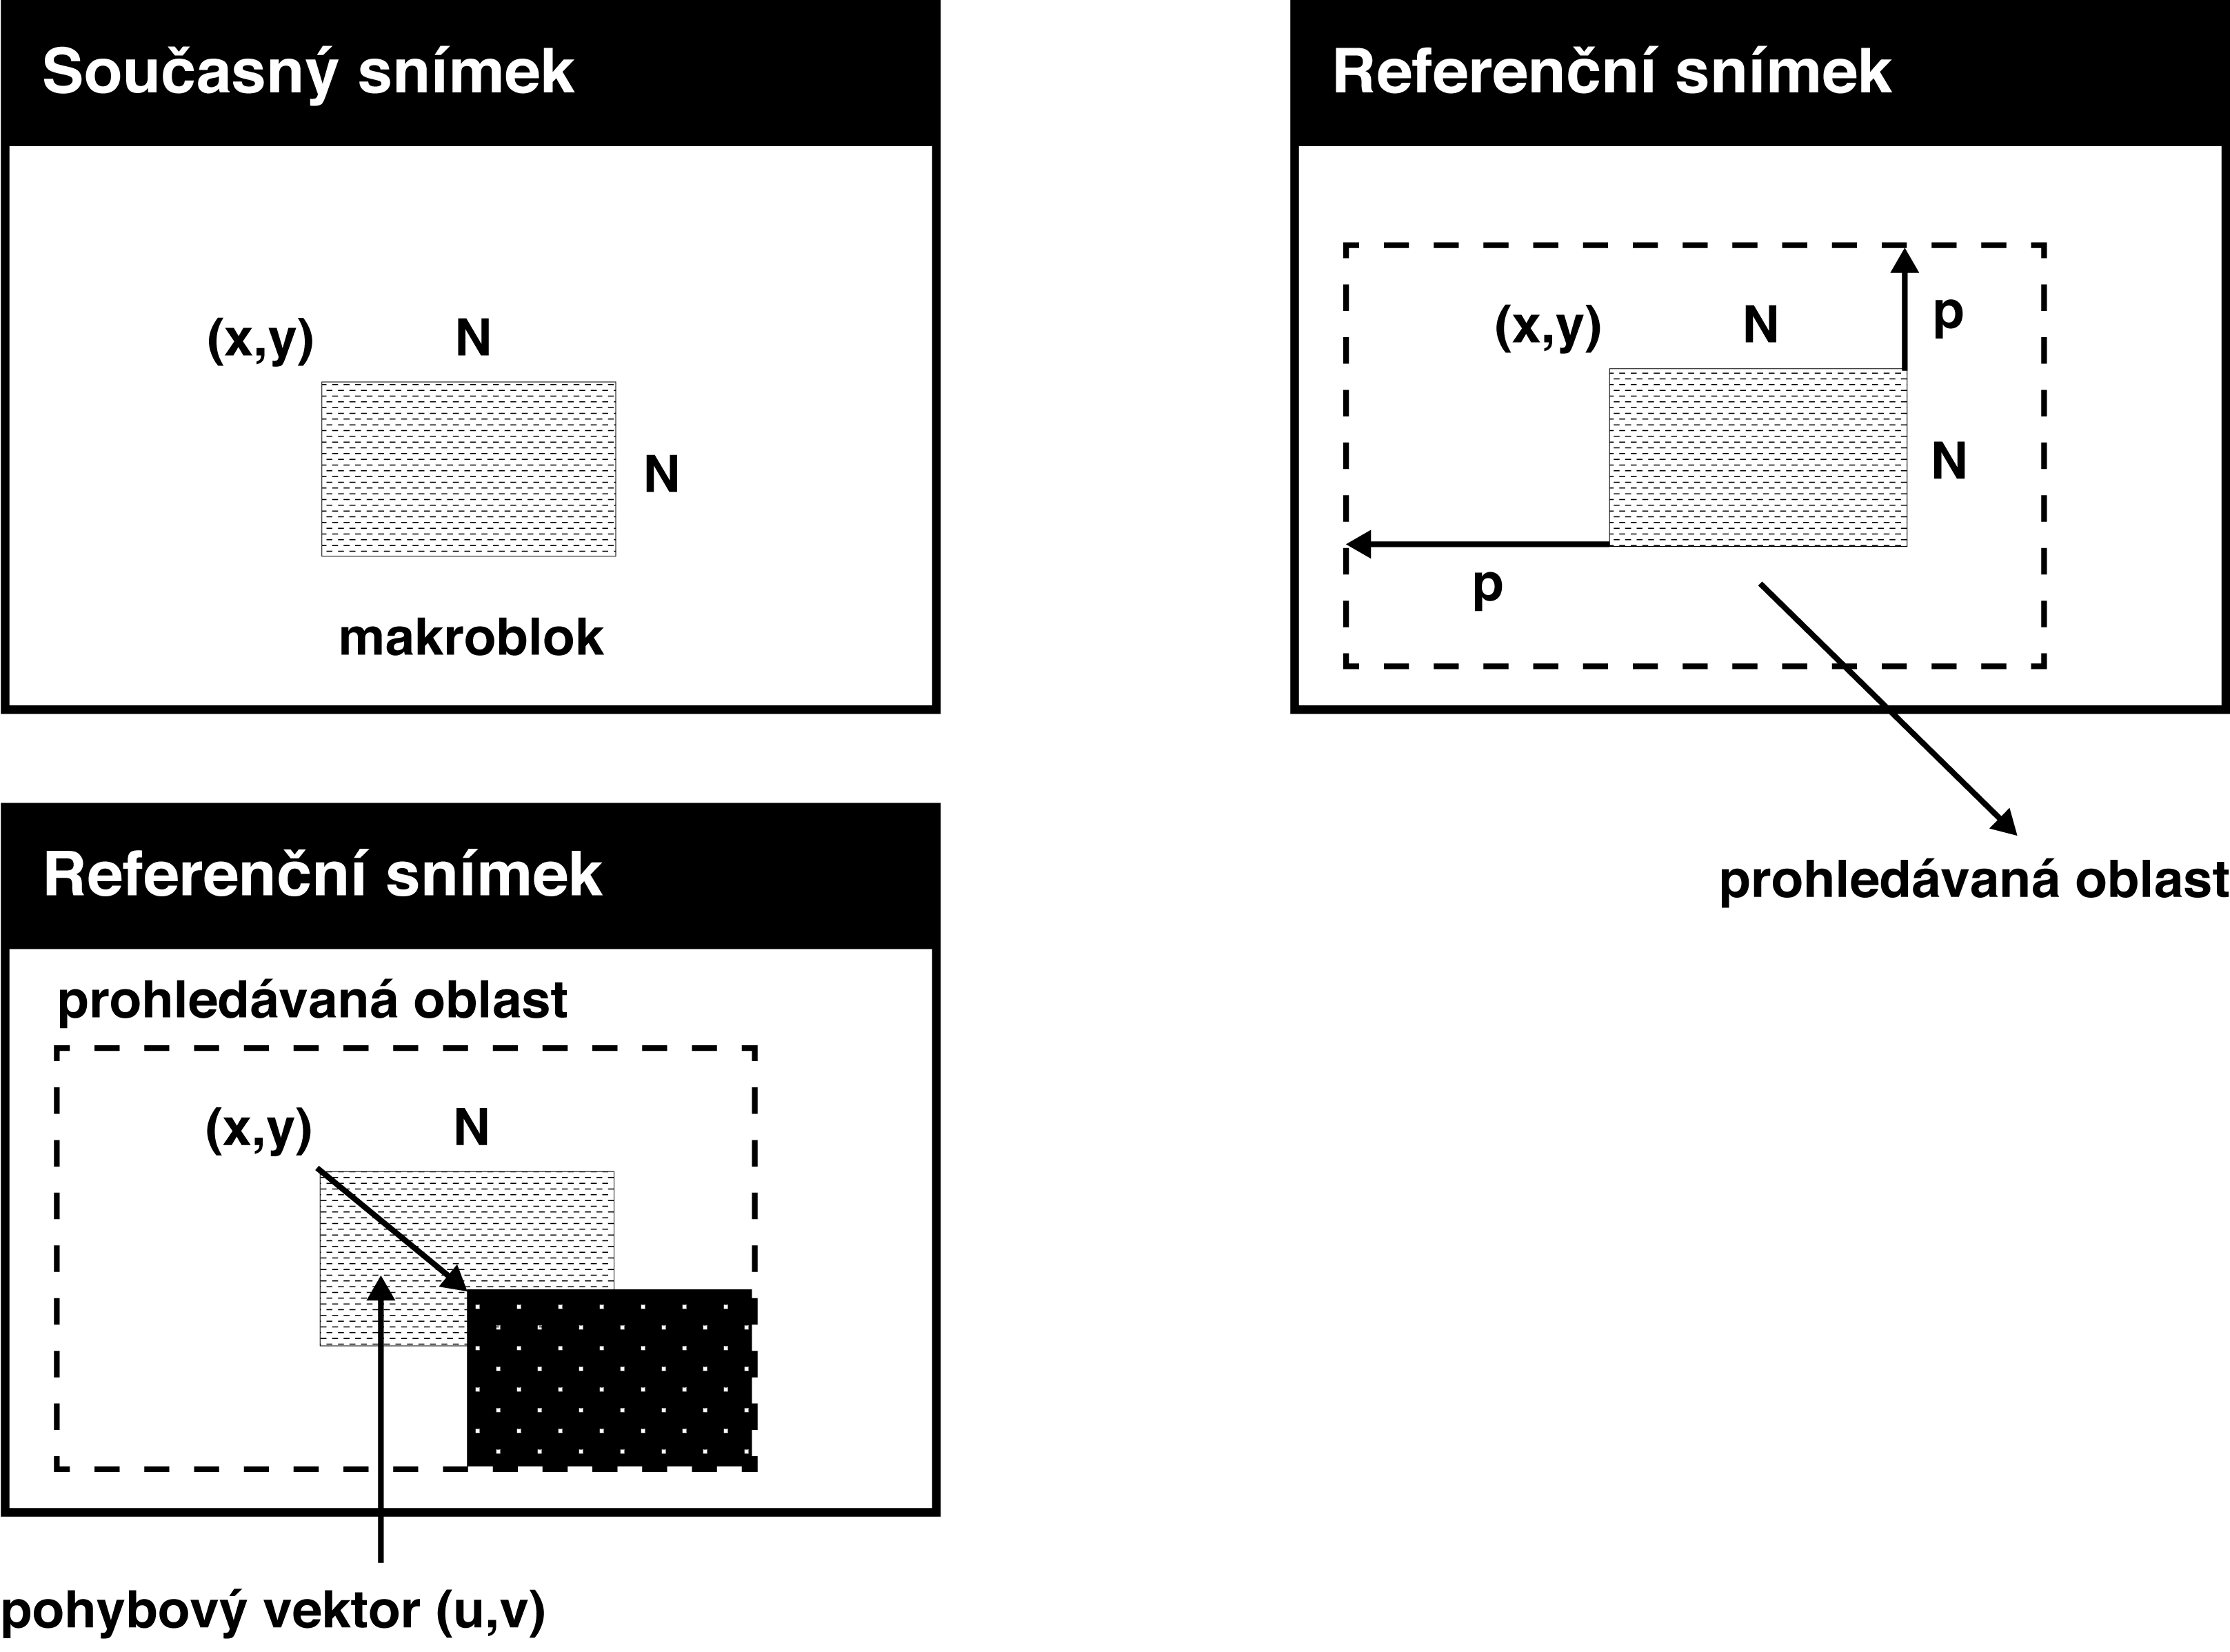
\includegraphics[scale=0.5]{obrazky/makroblok.png}
  \end{center}
  \caption{Hledání vektorů pohybu}
\end{figure}

\subsection*{Třída pro detekci pohybu z obrazu}

PiMotionAnalysis je třída poskytnutá knihovnou PiCamera pro detekci pohybu z obrazu v reálném čase, využívající metodu počítání vektorů pohybu.

Třída implementuje metodu analyse, která je volána pro každý snímek. V této metodě je nutné implementovat logiku počítání velikosti vektorů a prahování.

Práh detekce je možné parametrizovat minimální velikostí vektoru, tj. o kolik se daný makroblok posunul. A také počtem vektorů splňující danou minimální velikost.

Níže je ukázka výpočtu velikosti pohybových vektorů za použití modulu Numpy.

\begin{minted}[breaklines,frame=single]{python}
class vectorMotionAnalysis(picamera.array.PiMotionAnalysis):
    def analyse(self, a):
        a = np.sqrt(
            np.square(a['x'].astype(np.float)) +
            np.square(a['y'].astype(np.float))
            ).clip(0, 255).astype(np.uint8)
        # Jestli je více jak 10 vektorů s velikostí 
        # větší než 60, pohyb je detekován
        if (a > 60).sum() > 10:
            print('Pohyb detekován!')
\end{minted}

\section{Řízení snímání fotografií}
Řízení snímání fotografií je poskytnuto třídou CaptureHandler a metodou tick.

Metoda tick je volána každou sekundu.

Pokud je zavolána metoda motion\_detected a přitom současně není zpracovávána žádná jiná fotografie, provede se metoda tick.

\subsection*{Parametry snímaných fotografií}
Ve výchozím nastavení se snímá v rozlišením 640x368 pixelů.

Pro denní režim je nastavení módu expozice a vyvážení bílé automatické. Rychlost uzávěrky je také automatická. V nočním režimu je použit expoziční režim nightpreview a doba uzávěrky je nastavena na 200 ms.

Fotografie jsou zkomprimovány a optimalizovány za použití modulu PIL ve výchozím nastavením komprese 75.
\clearpage
\begin{minted}[frame=single]{python}
# Ukázka snímání fotografie v noci 
with picamera.PiCamera() as camera:
    camera.resolution = (1280, 720)
    # Snímkovací frekvence je nastavena na 1 fps 
    # Doba uzávěrky je nastavena na 200 milisekund a ISO na 800
    camera.framerate = 1
    camera.shutter_speed = 200000
    camera.exposure_mode = 'nightpreview'
    camera.iso = 800
    # Kamera potřebuje čas na změření AWB - Auto white balance
    sleep(10)
    camera.capture('dark.jpg')
    # Snímek je pořízen
\end{minted}

\subsection*{Detekci denní doby}
Detekce intenzity osvětlení (respektive denní doby) je řešena softwarově.

Využívá se výpočtu průměrné hodnoty pixelů vyjádřené v RGB.

Tato metoda není příliš přesná, ale je dostačující pro rozhodnutí, zda-li má být fotografie pořízena v nočním režimu s přísvitem.

Měří se průměrná hodnota pixelu v testované matici.

Experimentálně bylo zjištěno, že pokud je průměrná hodnota vyšší jak 100, můžeme prohlásit, že světelné podmínky jsou dostatečné pro použití parametrů pro denní snímání.

\begin{minted}[breaklines,frame=single]{python}
def scanIfDay():
    with picamera.PiCamera() as camera:
        camera.resolution = (testWidth, testHeight)
        with picamera.array.PiRGBArray(camera) as stream:
            camera.exposure_mode = 'auto'
            camera.awb_mode = 'auto'
            camera.capture(stream, format='rgb')
            pixAverage = int(np.average(stream.array[...,1]))
    logging.info("Light Meter pixAverage=%i" % pixAverage)
    if (pixAverage > 100):
        return True
    else:
        return False
\end{minted}




\subsection*{Vývojový diagram detekce pohybu}

\usetikzlibrary{positioning, shapes.geometric, arrows}

\tikzstyle{startstop} = [rectangle, rounded corners, minimum width=3cm, minimum height=1cm,text centered, draw=black]
\tikzstyle{io} = [trapezium, trapezium left angle=70, trapezium right angle=110, minimum width=3cm, minimum height=1cm, text centered, draw=black]
\tikzstyle{process} = [rectangle, minimum width=3cm, minimum height=1cm, text centered, text width=3cm, draw=black]
\tikzstyle{decision} = [diamond, minimum width=3cm, minimum height=1cm, text centered, text width=3cm, draw=black]
\tikzstyle{arrow} = [thick,->,>=stealth]
\begin{tikzpicture}[node distance=2.5cm]

%Nodes
\node (start) [startstop] {Start};
%\node (in1) [process, below of=start] {Načtení %konfiguračního souboru JSON};
\node (promod) [process, below of=start] {Volba módu};
\node (dec1) [decision, below of=promod, yshift=-0.5cm] {Je noc?};
\node (pro1a) [process, below of=dec1, yshift=-1cm] {Denní snímání};
\node (pro1b) [process, right of=dec1, xshift=3cm] {Noční snímání};
\node (pro2) [process, below of=pro1a] {Pořízení fotografie};
\node (pro3) [io, below of=pro2] {Zkomprimovat a uložit na SD kartu};
\node (out1) [io, below of=pro3] {Vložení fotografie do fronty na upload};
\node (stop) [startstop, below of=out1] {Stop};

%Arrows
%\draw [arrow] (start) -- (in1);
%\draw [arrow] (in1) -- (promod);
\draw [arrow] (start) -- (promod);
\draw [arrow] (promod) -- (dec1);
\draw [arrow] (dec1) -- node[anchor=east] {False} (pro1a);
\draw [arrow] (dec1) -- node[anchor=south] {True} (pro1b);
\draw [arrow] (pro1b) -- (pro2);
\draw [arrow] (pro1a) -- (pro2);
\draw [arrow] (pro2) -- (pro3);
\draw [arrow] (pro3) -- (out1);
\draw [arrow] (out1) -- (stop);

\end{tikzpicture}



\clearpage
\section{Detekce pohybu z PIR pomocí obsluhy přerušení}
Ukázka řešení detekce pohybu ze senzoru PIR pomocí obsluhy přerušení.

Obsluha přerušení je řešena pomocí modulu GPIO.

PIR senzor je připojen k GPIO pinu 7.

\begin{minted}[breaklines,frame=single]{python}
import RPi.GPIO as GPIO
import time

GPIO.setmode(GPIO.BCM)  # nastav mod cislovani na BCM
PIR_PIN = 7             # nastaveni PIR na pin 7 (BCM)
GPIO.setup(PIR_PIN, GPIO.IN) # nastavime pin na vstupni

def MOTION(PIR_PIN):
    print("Detekovan pohyb!")

print ("Test PIR senzoru") # pockame na inicializaci
time.sleep(2)
print("Pripraven")

try:
    GPIO.add_event_detect(PIR_PIN, GPIO.RISING, callback=MOTION) 

while 1:
    time.sleep(100)

except KeyboardInterrupt:
    print("Konec") # ukonceni na preruseni z klavesnice
    GPIO.cleanup()

\end{minted}

\clearpage

\section*{Odesílání fotografií na cloudové úložiště}
Po nasnímání jsou fotografie zkomprimovány a optimalizovány s použitím JPEG podle nastavené úrovně komprese a uloženy na lokální úložiště.

Jméno fotografie je časová známka v době, kdy byla pořízena.

Toto jméno souboru fotografie je následně vloženo do fronty, která je sdílena s vláknem pro odesílání fotografií, ve kterém je v daných časových intervalech vyčítána a nezávisle na běhu hlavního vlákna je posílána do vzdáleného úložiště.

\section{Ovládání aplikace}

\subsection*{Ovládací panel aplikace}

Ovládací panel je řešen prostřednictvím aplikace Google Sheets pomocí Google API, která umožňuje integraci aplikací napsaných v jazyce Python s produkty Google.

K tomuto řešení bylo přistoupeno z důvodu požadavku na vzdálenou konfiguraci aplikace bez nutnosti provozovat nějaký webový server pro běh rozhraní.

Google API je tzv. REST, to znamená, že je implementováno na protokolu HTTP.

Z toho plynoucí výhody jsou jednoduchost implementace a malý přenášený objem dat. Jsou přenášena pouze ta data, která jsou vyžádána.

V neposlední řadě je to také spolehlivost a rychlost zajištěná servery Google a také možnost publikace celého dokumentu veřejně přístupnou HTML stránkou. 

Rozhraní vytvořené pro aplikaci obsahuje pět sešitů.

Úvodní sešit nazvaný Dashboard obsahuje grafické shrnutí údajů o stavu nabíjení a napájení a také o stavu systémových prostředků jako je vytížení CPU a RAM.

Data, ze kterých se vychází, se ukládají do sešitu zvaném Log.

V dalším sešitu jsou zobrazeny náhledy fotografií nasnímaných při detekci pohybu.

Následující sešit obsahuje log zpráv, označených jmény vláken, odkud zprávy přišly.

Zprávy jsou řazeny do čtyř kategorií:
\begin{itemize}
    \item DEBUG - podrobné informace o chodu programu, je možné je vypnout. 
    \item INFO - informační zprávy.
    \item WARNING - varování neohrožující chod programu.
    \item ERROR - chyby.
    \item CRITICAL - velmi závážné chyby, které znemožňují chod programu.
\end{itemize}

Poslední sešit umožňuje konfigurovat zařízení pomocí dialogového okna s formulářem.

Na základě zadaných dat je vygenerován konfigurační soubor ve formátu JSON, který je poté stažen ve vlákně pro kontrolu konfigurace.

\begin{figure}[h]
  \begin{center}
    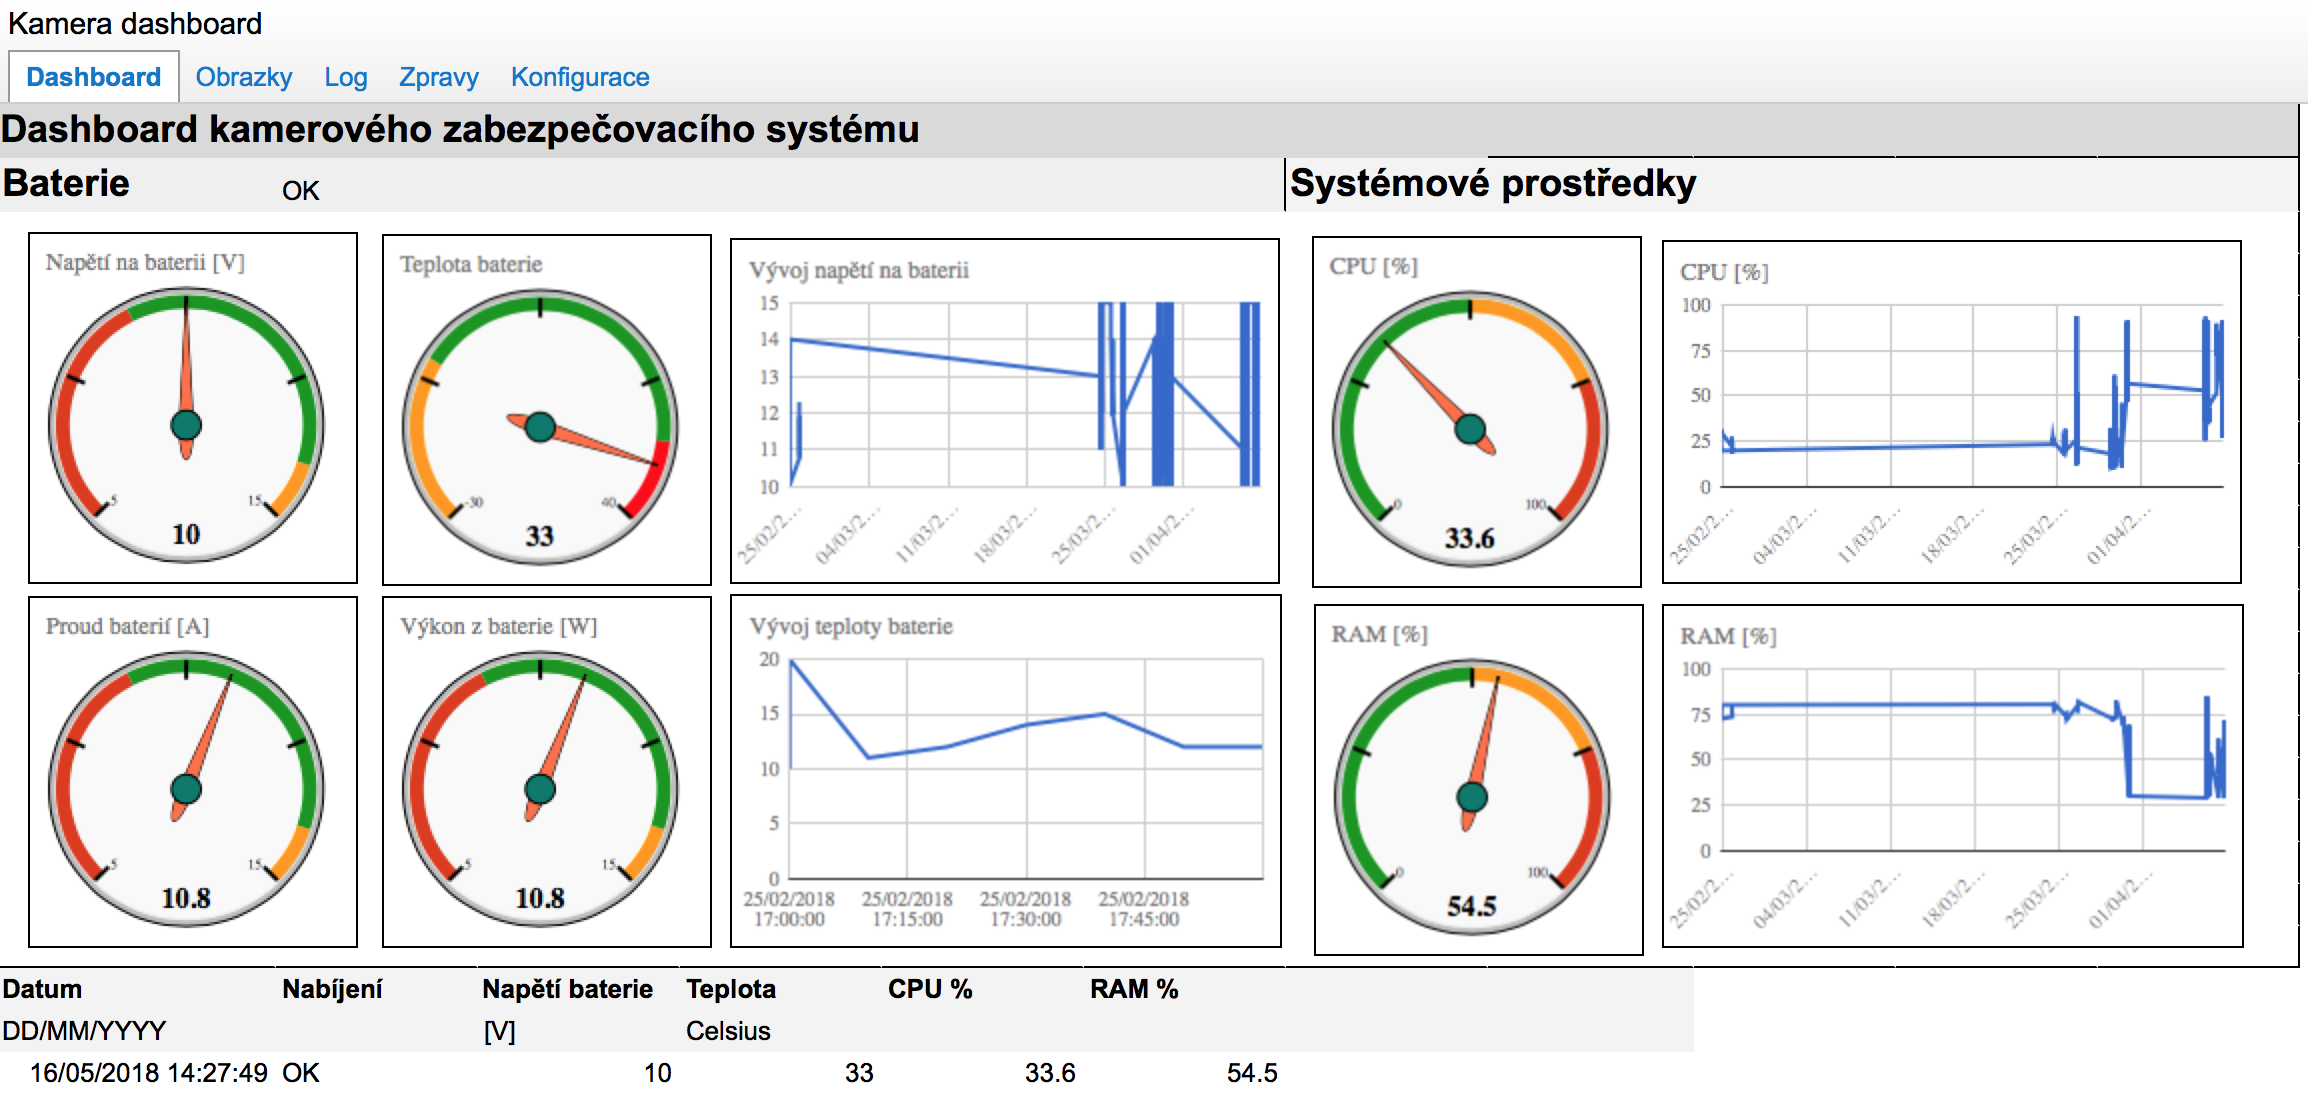
\includegraphics[scale=0.3]{obrazky/dashboard2.png}
  \end{center}
  \caption{Informační panel aplikace}
\end{figure}

\begin{figure}[h]
  \begin{center}
    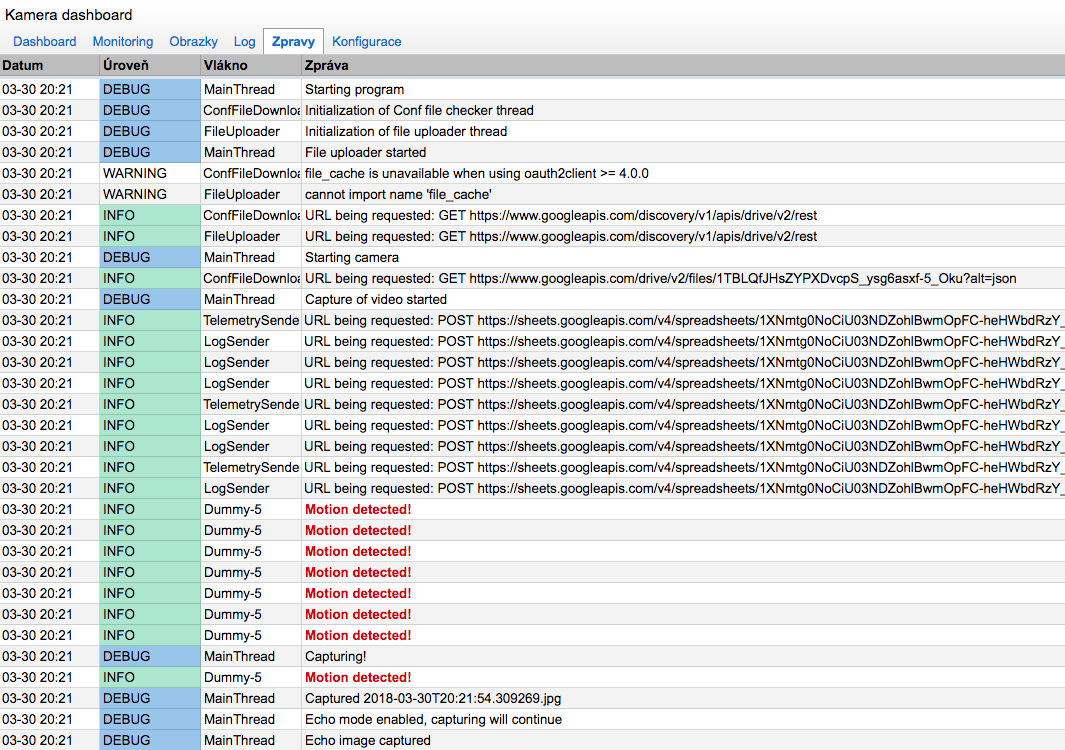
\includegraphics[scale=0.35]{obrazky/logy.png}
  \end{center}
  \caption{Panel aplikace obsahující log}
\end{figure}

\subsection*{Ovládání a notifikace pomocí SMS}

Aplikaci je možné ovládat pomocí SMS z jednoho autorizovaného čísla, pokud je v konfiguračním souboru nastavený parametr SMS control.


\begin{table}[h]
\centering
\caption{Příkazy SMS}
\label{sms}
\begin{tabular}{|l|l|l|}
\hline
\textbf{SMS příkaz} & \textbf{Popis}            & \textbf{Odpověď} \\ \hline
BATTERY             & Informace o stavu baterie & Charging 12.3V     \\ \hline
TAKEPHOTO           & Okamžitá fotografie       &   -               \\ \hline
SET MODE <x>          & Nastav mód na x           & Mode has been set to <x>     \\ \hline
Q MODE              & Dotaz na aktivní mód      & Current mode is <x>     \\ \hline
 -                   & Nesprávný příkaz     &   Command not recognized                \\ \hline

\end{tabular}
\end{table}

\subsection*{Notifikace pomocí emailu}

Upozornění na detekci pohybu je také odesláno e-mailem prostřednictvím Google Cloud.

Kontrola nových fotografií na Google Drive je spouštěna každou minutu.

Pokud jsou detekovány nové fotografie, tak je odeslán e-mail na zvolenou e-mailovou adresu spolu s fotografiemi, které byly pořízeny. Následně se aktualizuje seznam fotografií v sešitu.


\section{Konfigurace}

Konfigurační data jsou v rámci aplikace uloženy ve dvou třídách - BaseConfig a UserConfig. Vzdáleně měnit je možné pouze konfigurace třídy UserConfig.

Konfigurace je načítána ze souboru ve formátu JSON, který je umístěn na úložišti Google Drive. Po stažení je zahájena kontrola a parsování souboru do třídy UserConfig.

Konfigurační soubor je v určitých intervalech dotazován na změnu. Pokud byl konfigurační soubor změněn, je stažen a načten. Toto je řešeno ve vlákně ConfFileDownloader.

\subsection*{Režim detekce}
Aplikace pracuje ve čtyřech základních režimech.
\begin{itemize}
    \item Real-time
    \item Batch
    \item On-demand
    \item Interval
\end{itemize}

\subsection*{Real-time režim}
V tomto režimu se fotografie pořídí ihned, jakmile je detekován pohyb.

Fotografie je také ihned odeslána na úložiště. Volitelně je pak možné zapnout upozornění SMS zprávou na zadané telefonní číslo a tzv. „dozvuk“, kdy se bude pokračovat ve snímkování každou sekundu i po prvotní detekci pohybu po následujících deset sekund.

Režim má v JSON konfiguračním souboru pod paremetrem \textit{mode} přiřazenou hodnotu \textit{realtime}.

\subsection*{Batch režim}
Tento režim funguje obdobně jako režim Real-time. Snímky však nejsou odeslány ihned po detekci pohybu, ale pouze jednou denně ve zvolené době.

Volitelně je pak možné zapnout upozornění SMS zprávou na zadané telefonní číslo a tzv.  „dozvuk“, kdy se bude pokračovat ve snímkování i po detekci pohybu v zadaném intervalu.

Režim má v JSON konfiguračním souboru pod paremetrem \textit{mode} přiřazenou hodnotu \textit{batch}.

\subsection*{On-demand}
On-demand, neboli na vyžádání, je režim, kdy se fotografie pořídí pouze na vyžádání pomocí SMS zprávy.

Režim má v JSON konfiguračním souboru pod paremetrem \textit{mode} přiřazenou hodnotu \textit{demand}.

\subsection*{Interval}
Tento režim umožňuje nastavení pravidelného snímkování v daném intervalu. Interval se nastavuje v minutách pomocí parametru interval.

Režim má v JSON konfiguračním souboru pod paremetrem \textit{mode} přiřazenou hodnotu \textit{interval}.

\subsection*{Režim echo}
Režim echo je volitelným parametrem pro nastavení „dozvuku“, tj. snímání dalších deseti fotografií po první detekci v sekundových intervalech.

\subsection*{Konfigurační soubor}
Parametrem \textit{mode} se nastavuje pracovní režim detekce, jsou povoleny čtyři hodnoty: \textit{realtime, batch, demand a interval}.

Parametr \textit{echo} je volitelným parametrem pro nastavení  „dozvuku“, tj. snímání fotografií ve stanoveném intervalu po první detekci a uplatňuje se pouze pokud je zvolen režim real-time nebo batch.

Parametr \textit{interval} nastavuje interval snímkování pro režim interval. Je zadáván v sekundách.

Ovládání a notifikace pomocí SMS zpráv je upravena parametry \textit{SMS\_notification}, \textit{SMS\_control} a \textit{authorized\_numbers}. Pole \textit{authorized\_number} obsahuje telefonní číslo, které může ovládat zařízení pomocí SMS příkazů a zároveň dostáví notifikace.

K datovému typu string bylo přistoupeno z důvodu lepší serializace z HTML formulářů.

\begin{table}[h]
\centering
\caption{Parametry konfiguračního souboru}
\label{}
\begin{tabular}{|l|l|l|}
\hline
\textbf{Parametr}  & \textbf{Datový typ} & \textbf{Popis}                 \\ \hline
mode               & string              & Metoda detekce                 \\ \hline
echo               & string             & Použití dozvuku        \\ \hline
interval              & number             & Interval        \\ \hline
SMS\_notification  & string             & Notifikace pomocí SMS          \\ \hline
SMS\_control       & string             & Ovládání pomocí SMS            \\ \hline
authorized\_number & string              & Autorizované číslo              \\ \hline
\end{tabular}
\end{table}

\begin{minted}[frame=single]{json}
{
	"mode": "realtime",
	"echo": "off",
	"interval": 5,
	"use_pir": "on",
	"SMS_notification": "off",
	"SMS_control": "on",
	"authorized_number": "+420733122122"
}
\end{minted}

\clearpage
\subsection*{Rozhraní pro konfiguraci}

Rozhraní pro konfiguraci je poskytnuto jako nadstavba nad Google Sheets vytvořená pomocí HTML a JavaScriptu. Samotná konfigurace se provádí v uživatelsky přívětivém formuláři. Po odeslání se pomocí JavaScriptu serializují data uložena ve formuláři do podoby JSON - JavaScript Object Notation a následně se uloží na Google Drive.

\begin{figure}[h]
  \begin{center}
    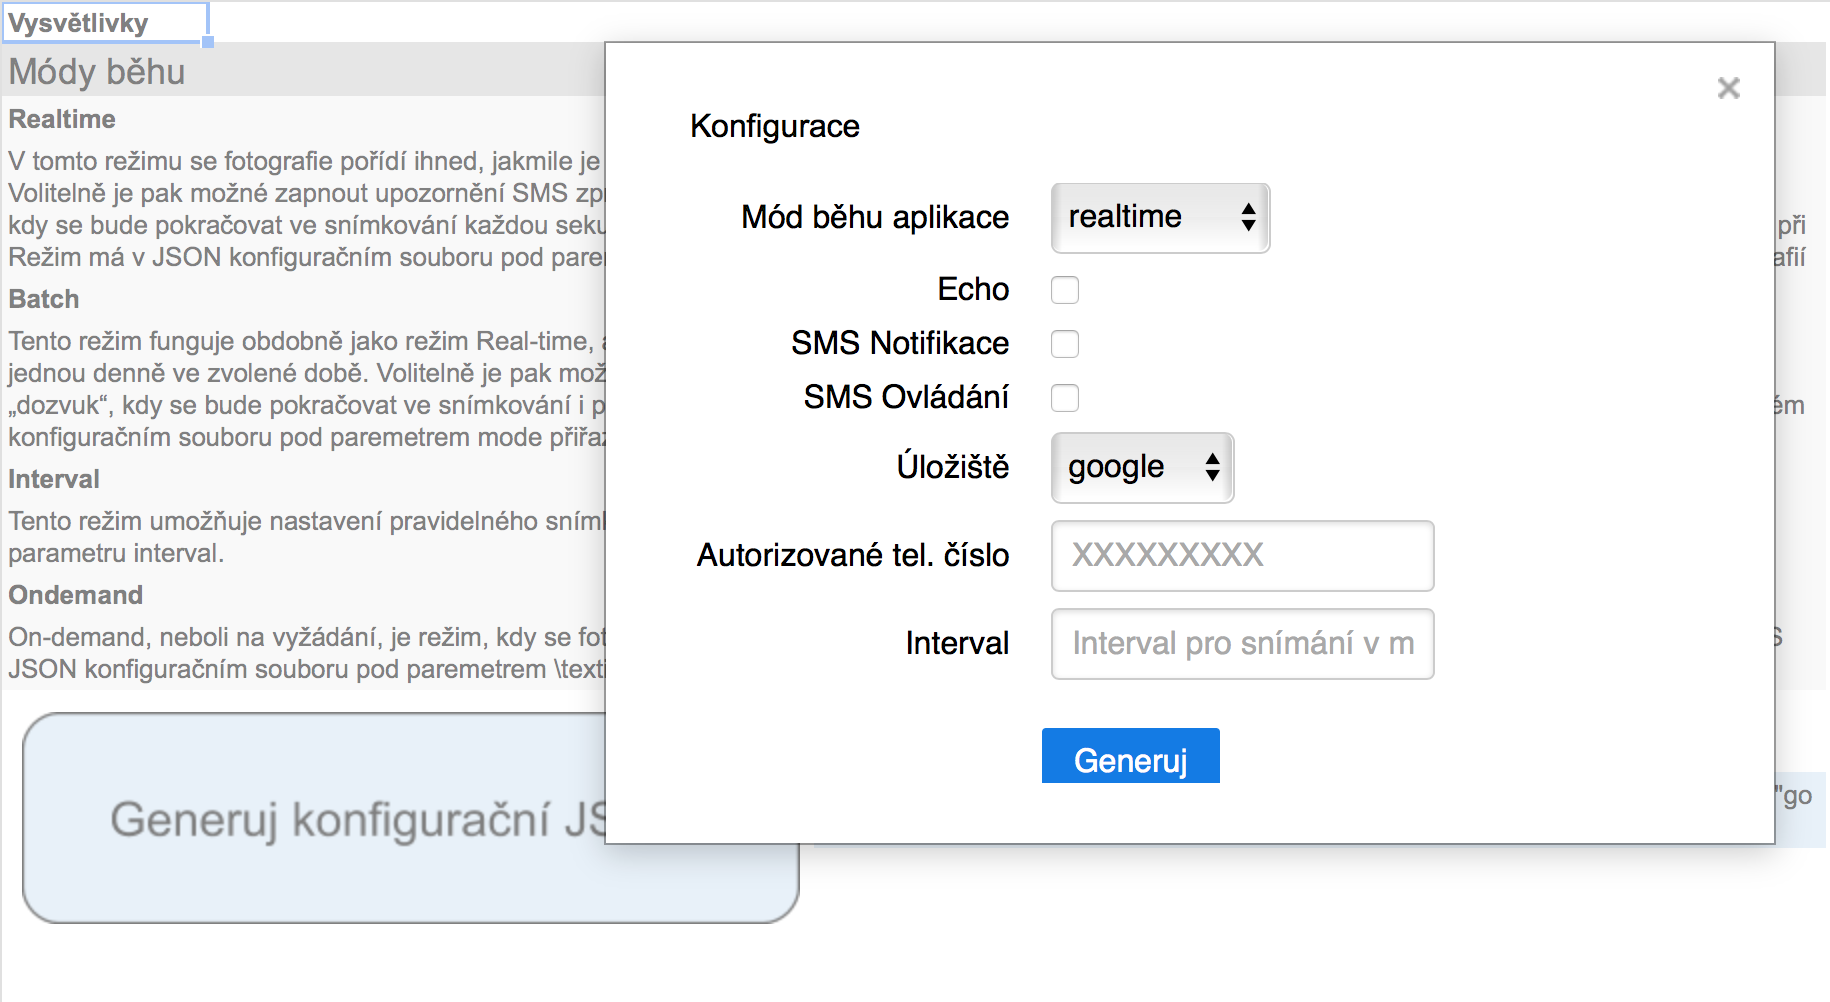
\includegraphics[scale=0.35]{obrazky/konfigurace.png}
  \end{center}
  \caption{Rozhraní pro konfiguraci}
\end{figure}


\section{Sledování stavu baterie}

Vyčítání stavu baterie a průběhu nabíjení ze solárního regulátoru Epsolar LS1024B je možné realizovat pomocí rozšiřujícího modulu epsolar-tracer, který umožňuje vyčítat následující informace: napětí baterie, napětí na solárním panelu, proud na zátěži, nabíjecí proud a teplotu baterie.

Komunikace je realizována pomocí protokolu Modbus.
\clearpage

\chapter{Návrh zapojení}

\section{Prototypování}

Před samotným návrhem výsledného zařízení, je vhodné nejprve komponenty sestavit na nepájivém poli abychom otestovali vzájemnou funkčnost a případně odstranili nedostatky.

\begin{figure}[h]
  \begin{center}
    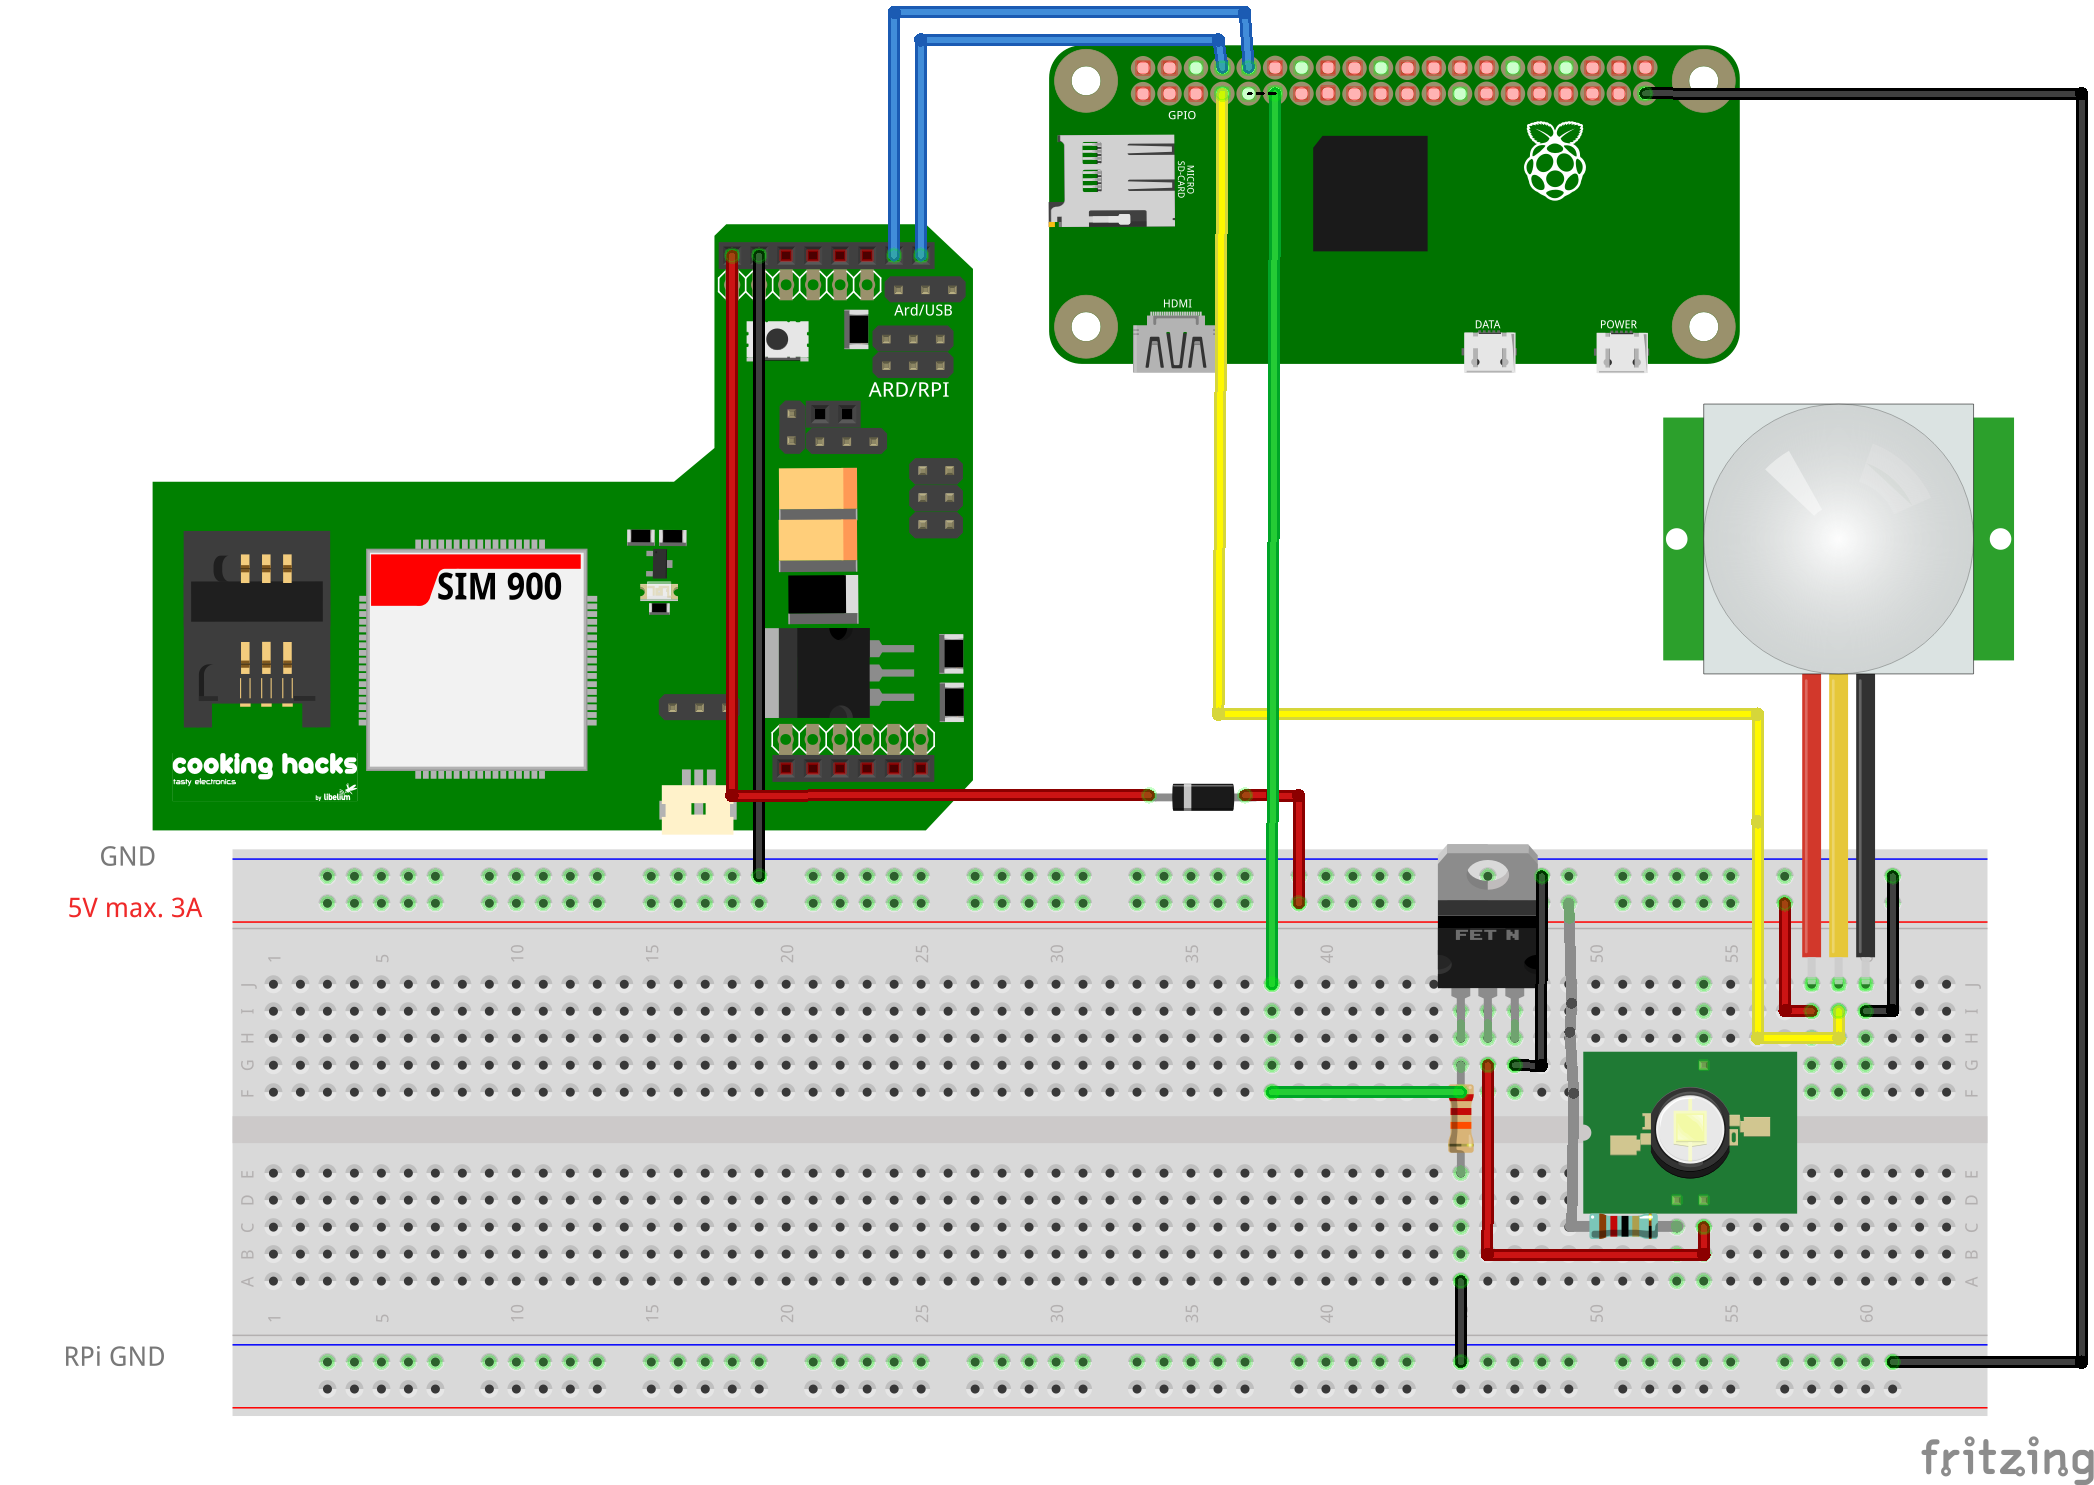
\includegraphics[scale=0.75]{obrazky/schema.png}
  \end{center}
  \caption{Prototyp zařízení sestavený na nepájivém poli}
\end{figure}

\section{Řešení napájení}
\subsubsection{Spotřeba zařízení}
Před samotným návrhem napájecího obvodu je nutné nejprve zjistit proudový odběr jednotlivých komponent zařízení z katalogů.

% Please add the following required packages to your document preamble:
% \usepackage{multirow}
%\begin{table}[]
%\centering
%\caption{My caption}
%\label{my-label}
%\begin{tabular}{|l|l|l|l|}
%\hline
%\multirow{2}{*}{\textbf{Komponenta}} & %\multicolumn{3}{l|}{\textbf{Proudový odběr {[}mA{]}}} \\ \cline{2-4} 
%                                     & \textit{minimum}  & %\textit{typická}  & \textit{max}  \\ \hline
%RPi Zero W                           & 80                & 150           %    & 240           \\ \hline
%RPi Camera v2.1                      & 100               & 100           %    & ?             \\ \hline
%SIM900                               & 1,5               & -             %    & 2000          \\ \hline
%PIR senzor                           & -                 & 65            %    & -             \\ \hline
%LED                                  & -                 & 400           %    & 420           \\ \hline
%\end{tabular}
%\end{table}
\subsubsection{Napájení Raspberry Pi Zero W}
Špičkový proudový odběr samotného Raspberry Pi Zero W může dosahovat až 350 mA. Výrobce doporučuje použít zdroj, který je schopen dodávat 700 mA. 

Raspberry Pi je možné napájet z USB portu, nebo přes GPIO 5 V pin. V případě GPIO je nutné zajistit stabilní napájení, protože pin je zapojen přímo na 5voltovou větev bez filtračního obvodu.

V našem případě můžeme Raspberry Pi napájet z GPIO, protože máme zajištěné stabilní napětí a ochranu z DC-DC měniče.

\begin{figure}[h]
  \begin{center}
    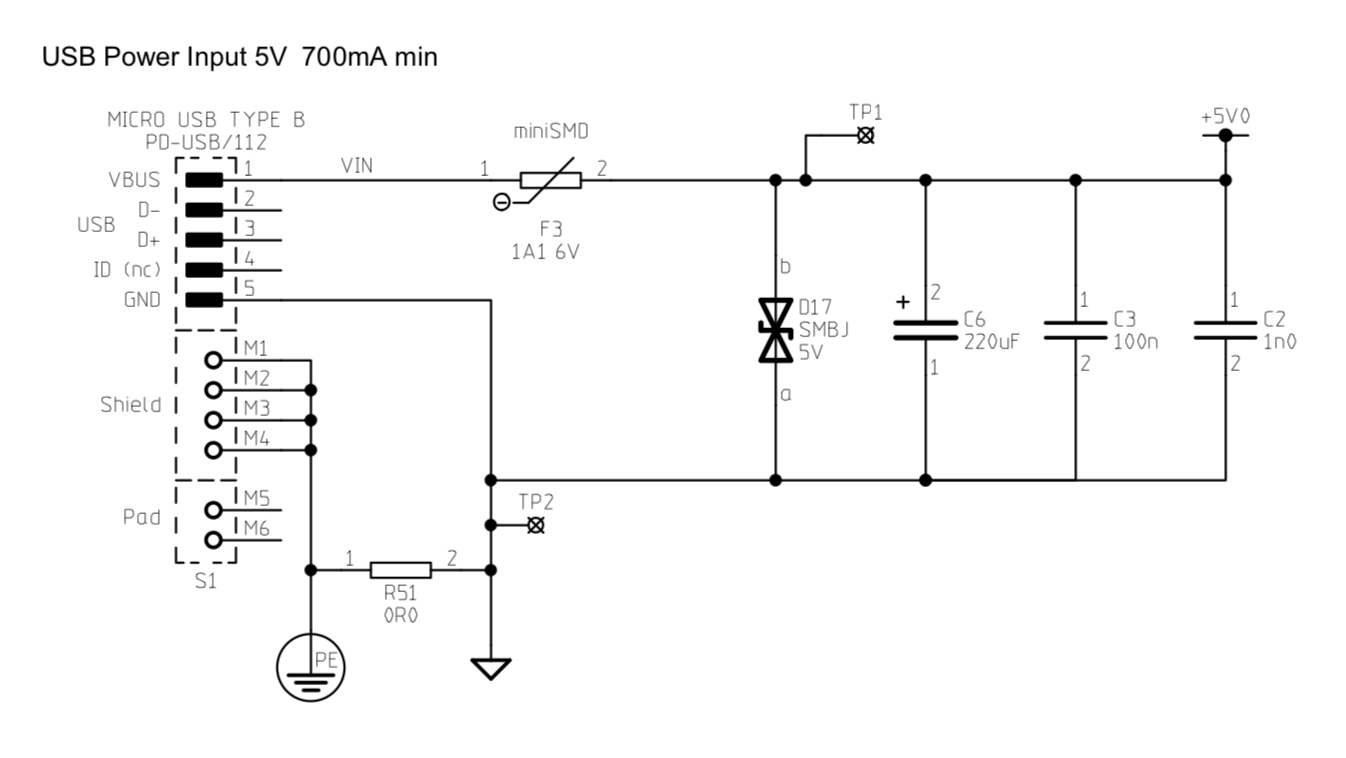
\includegraphics[scale=0.5]{obrazky/rpi_power.png}
  \end{center}
  \caption{Schéma napájení RPi přes USB, zdroj raspberrypi.org}
\end{figure}

\subsubsection{Napájení modulu SIM800}
Špičkový proudový odběr modulu SIM800 může dosahovat až 2 A při 5 V, zejména při registraci do sítě. Bude tedy nutné napájení dostatečně dimenzovat.

\begin{table}[h]
\centering
\caption{Proudový odběr komponent}
\label{my-label}
\begin{tabular}{|l|l|l|l|}
\hline
\textbf{Proudový odběr @5V {[}mA{]}} & \textit{min.} & \textit{typická} & \textit{max.} \\ \hline
RPi Zero W                       & 80               & 150              & 350          \\ \hline
RPi Camera v2.1                  & 100              & 100              & ?            \\ \hline
SIM800                           & 1,5              & -                & 2000         \\ \hline
PIR senzor                       & -                & -                & 65            \\ \hline
LED                              & -                & 400              & 420          \\ \hline
\end{tabular}
\end{table}

\subsubsection{Napájení výkonové LED}
Použitá výkonová LED dioda má proudový odběr 400 mA. Takový proud není možné poskytnout přes GPIO, bude nutné diodu spínat tranzistorovým spínačem. V úvahu ještě připadá spínat diodu pulzně přes PWM, ale bylo by nutné vyřešit problém s načasováním spouštění diody a pořizováním fotografií, aby nedocházelo ke stroboskopickému jevu.

\subsubsection{Návrh spínače výkonové LED}
Proudový odběr použité diody je 400 mA, úbytek napětí je 1,7 V. Diodu budeme spínat přes GPIO, které používá 3,3voltovou logiku. Prahové napětí pro sepnutí tranzistoru bude muset být minimálně 2,7 V, přičemž při napětím menším než 0,8 V musí být tranzistor zavřený. V úvahu připadá spínat LED diodu proudově řízeným bipolárním tranzistorem, nebo napěťově řízeným tranzistorem typu MOSFET. U tranzistoru typu MOSFET dochází k menším energetickým ztrátám než u bipolárního tranzistoru, ale vzhledem k vyšší ceně a malé dostupnosti výkonových logických tranzistorů pro 3,3voltovou logiku bude lepší použít Darlingtonovo zapojení bipolárních tranzistorů. Takový tranzistor má velké proudové zesílení a malý vstupní proud. 

V práci je použito tranzistorové pole ULN2003A sestávající ze sedmi Darlingtonových tranzistorů. K této součástce bylo přistoupeno z důvodu možného budoucího rozšíření o spínání více LED.  

\begin{figure}[h!]
  \begin{center}
    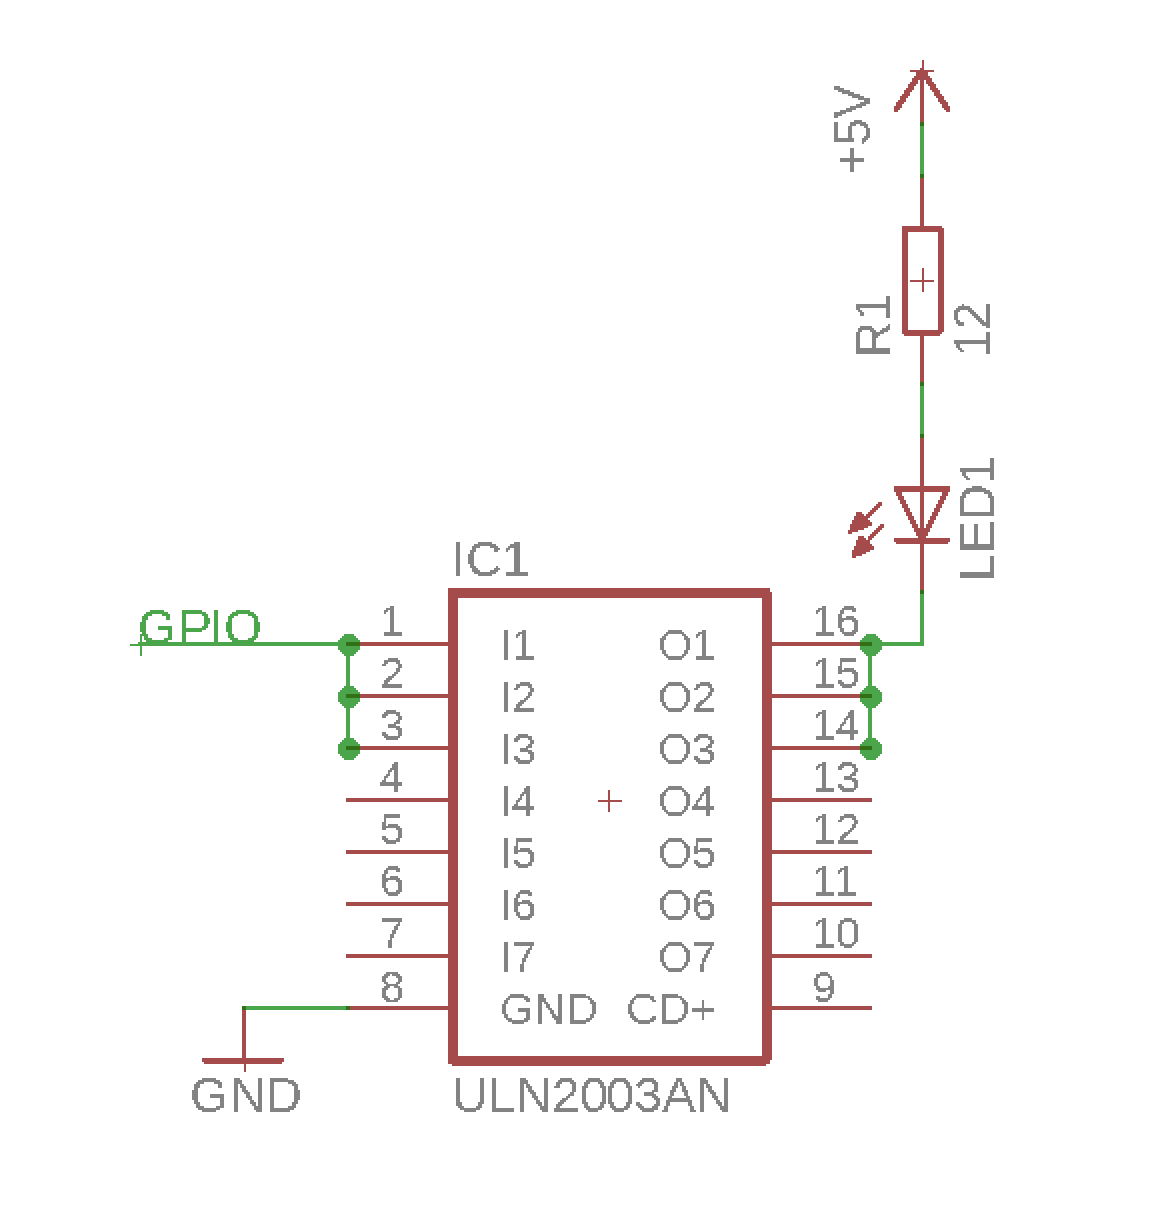
\includegraphics[scale=0.5]{obrazky/schema_switch2.png}
  \end{center}
  \caption{Schéma spínače výkonové LED}
\end{figure}


\subsection*{Solární panel a akumulátor}
Vzhledem k rozvaze o proudovém odběru jednotlivých komponent budeme vycházet z celkového průměrného proudového odběru 300 mA. Celkový příkon je tedy $0.3\times5 = 1.5 \ \jedn{W}$. Budeme uvažovat geografickou polohu Brna.

\subsubsection{Solární panel}
Dle Solargis.info dopadá v Brně 1150 $\jedn{kWh/m^2}$ solárního záření za rok.

$$1150000/8760 \approx 131 \ \jedn{W/m^2} $$

Průměrně tedy v Brně dopadá 131 $\jedn{W/m^2}$, avšak efektivita solárních panelů se pohybuje kolem 15\%, to je $20\ \jedn{W/m^2}$. Předpokládejme, že ztratíme dalších 33\% při přenosu energie. Celkově tedy máme využitelnou energie pouhých $14\ \jedn{W/m^2}$.

\subsubsection{Výpočet velikosti solárního panelu}
$$\frac{1.5\ \jedn{W}}{14\ \jedn{W/m^2}} \approx 1071 \ \jedn{cm^2}$$

Aby zařízení bylo možné provozovat celoročně, musíme provést výpočet velikosti solárního panelu pro měsíc s nejméně slunečnými dny, tedy pro prosinec. Využijeme kalkulátor Solar Electricity Handbook \cite{solar} pro zjištění úhrnu slunečního záření za měsíc prosinec.
Bude tedy nutné velikost panelu přepočítat s ohledem na měsíc prosinec. V prosinci v Brně dopadá průměrně 1,41 $\jedn{kWh/m^2}$ za den. Obecně platí, že panel by měl být natočen směrem na jih pod úhlem 41 stupňů pro celoroční optimum efektivity solárního panelu.


$$1410/24 \approx 59 \ \jedn{W/m^2} $$

Po přepočtu efektivity solárního panelu a ztráty při přenosu získáme $6 \ \jedn{W/m^2}$

\subsubsection{Přepočet výpočtu velikosti solárního panelu pro měsíc prosinec}
$$\frac{1.5W}{6\ \jedn{W/m^2}} \approx 2500 \ \jedn{cm^2}$$

Pro celoroční napájení bude nutné zajistit panel velikosti alespoň $2500 \ \jedn{cm^2}$

Tomuto požadavku odpovídá solární panel WS-30/12V.

\subsubsection{Akumulátor}

Použitý akumulátor musí zajistit nepřetržité napájení zařízení po dobu dlouhých zimních nocí, zejména v měsíci prosinci a také po dobu špatného počasí. Budeme tedy předpokládat, že zařízení musí vydržet týden bez dobíjení.

S ohledem na  nevýhody lithiových baterií uvedené v kapitol 1.5, bude zde vhodnější použít olověnou baterii.

Výpočítáme kapacitu akumulátoru pro noční provoz v prosinci, předpokládejme délku noci 16 h. Předpokládáme proudový odběr 300 mA při 5V.
$$16h\times0.3A=4.8 \ \jedn{Ah}$$

Výpočet kapacity akumulátoru pro týden bez slunce. Předpokládáme proudový odběr 300 mA při 5V.
$$7 dní \times 24 \ \jedn{h} \times 0.3 \ \jedn{A} \approx 50.4 \ \jedn{Ah}$$

Mezi odpovídající komerčně nabízené akumulátory patří Westinghouse WA12200 12V/20Ah.

\subsubsection{DC-DC Měnič 12/5V}
Pro změnu 12 V ze vstupu akumulátoru na 5 V, které je vyžadováno pro napájení všech komponent zařízení, je použit DC-DC měnič CPT 120503 12/5V od firmy Current Logic. Maximální udávaný proudový odběr je 3 A. Udávaná účinnost je v rozmezí 90 až 94 procent. Měnič také obsahuje ochranu proti zkratu a také ochranu proti přetížení.

\subsubsection{Solární regulátor Epsolar LS1024B}
Solární regulátor řídí nabíjení akumulátoru ze solárního panelu a také chrání baterii před jejím přebitím i hlubokým vybitím. Existují dva typy solárních regulátorů - MPPT a PWM. PWM solární regulátory vyhovují svými parametry pro naši aplikaci, používají pulzně šířkovou modulaci k dosažení optimálního nabití baterie. 

Požadavkem na solární regulátor je schopnost dodávat proud minimálně 3 A při 5 V, možnost připojení 12 V olověné baterie a 12 V solárního panelu. Dalším požadavkem je možnost vyčítání dat o stavu nabití baterie a nízká pořizovací cena. 

Tyto požadavky splňuje PWM solární regulátor LS1024B od firmy Epsolar, který umožňuje odebírat až 10A ze solárního panelu a dodávat 10A do zátěže. Je také umožněna datová komunikace přes protokol Modbus, realizovaná sériovou sběrnicí RS-485.

Komunikace mezi Raspberry Pi a solárním regulátorem je možné realizovat knihovnou epsolar-tracer pomocí převodníku RS-485 na USB.

\section{Komunikace s GSM modulem SIM800}
Komunikace s GSM modulem je realizována na rozhraní UART. Raspberry Pi disponuje jednou hardwarovou periferií UART, která je dostupná na pinech 14 (TX) a 15 (RX). Modul SIM800 podporuje maximální bitovou přenosovou rychlost 460800 bit/s, ale při použití multiplexovacího protokolu  GSM0710 je výrobcem doporučená maximální přenosová rychlost 115200 bit/s.

\subsubsection{Multiplexovací protkol GSM0710}
Modul SIM800 disponuje pouze jedním hardwarovým rozhraním UART, to znamená, že standardně můžeme otevřít pouze jedno spojení. V této aplikace, ale bude nutné navázat minimálně dvě spojení - pro PPP a druhé spojení pro posílání a přijímání SMS zpráv. 

3GPP definuje standard 27.010 (GSM0710), který umožňuje provádět multiplexování na přenosové vrstvě, které rozdělí datové toky do takzvaných DLC (Data Link Channel). Takový logický kanál je možné používat separátně, je tedy možné navázat PPP připojení na jednom kanálu a na druhém kanálu naslouchat zda-li nepřišla zpráva SMS.

Podpora pro multiplexovací protokol GSM0710 standardně v Linuxu není, ale je možné ji zkompilovat a přidat do kernelu v podobě LKM (Loadable Kernel Module). V repozitáři Linux kernelu ji najdeme v podobě zdrojového kódu jazyka C - n\_gsm.c. Po načtení modulu do kernelu je do adresáře proc přidán soubor zařízení gsmtty, který ale ještě není možný použít jako terminál.

Abychom mohli zařízení používat jako terminál je nutné připojit takzvanou "line discipline", toto je řešeno přes program cmux (autorem je Nicolas Le Munchet), který byl upraven dle specifikací modulu SIM800.

\begin{figure}[!h]
  \begin{center}
    
\includegraphics[scale=0.3]{obrazky/simcom.png}
  \end{center}
  \caption{Schéma multiplexovacího protokolu GSM0710}
\end{figure}

\clearpage

\section{Blokové schéma návrhu zařízení}
\begin{figure}[!h]
  \begin{center}
    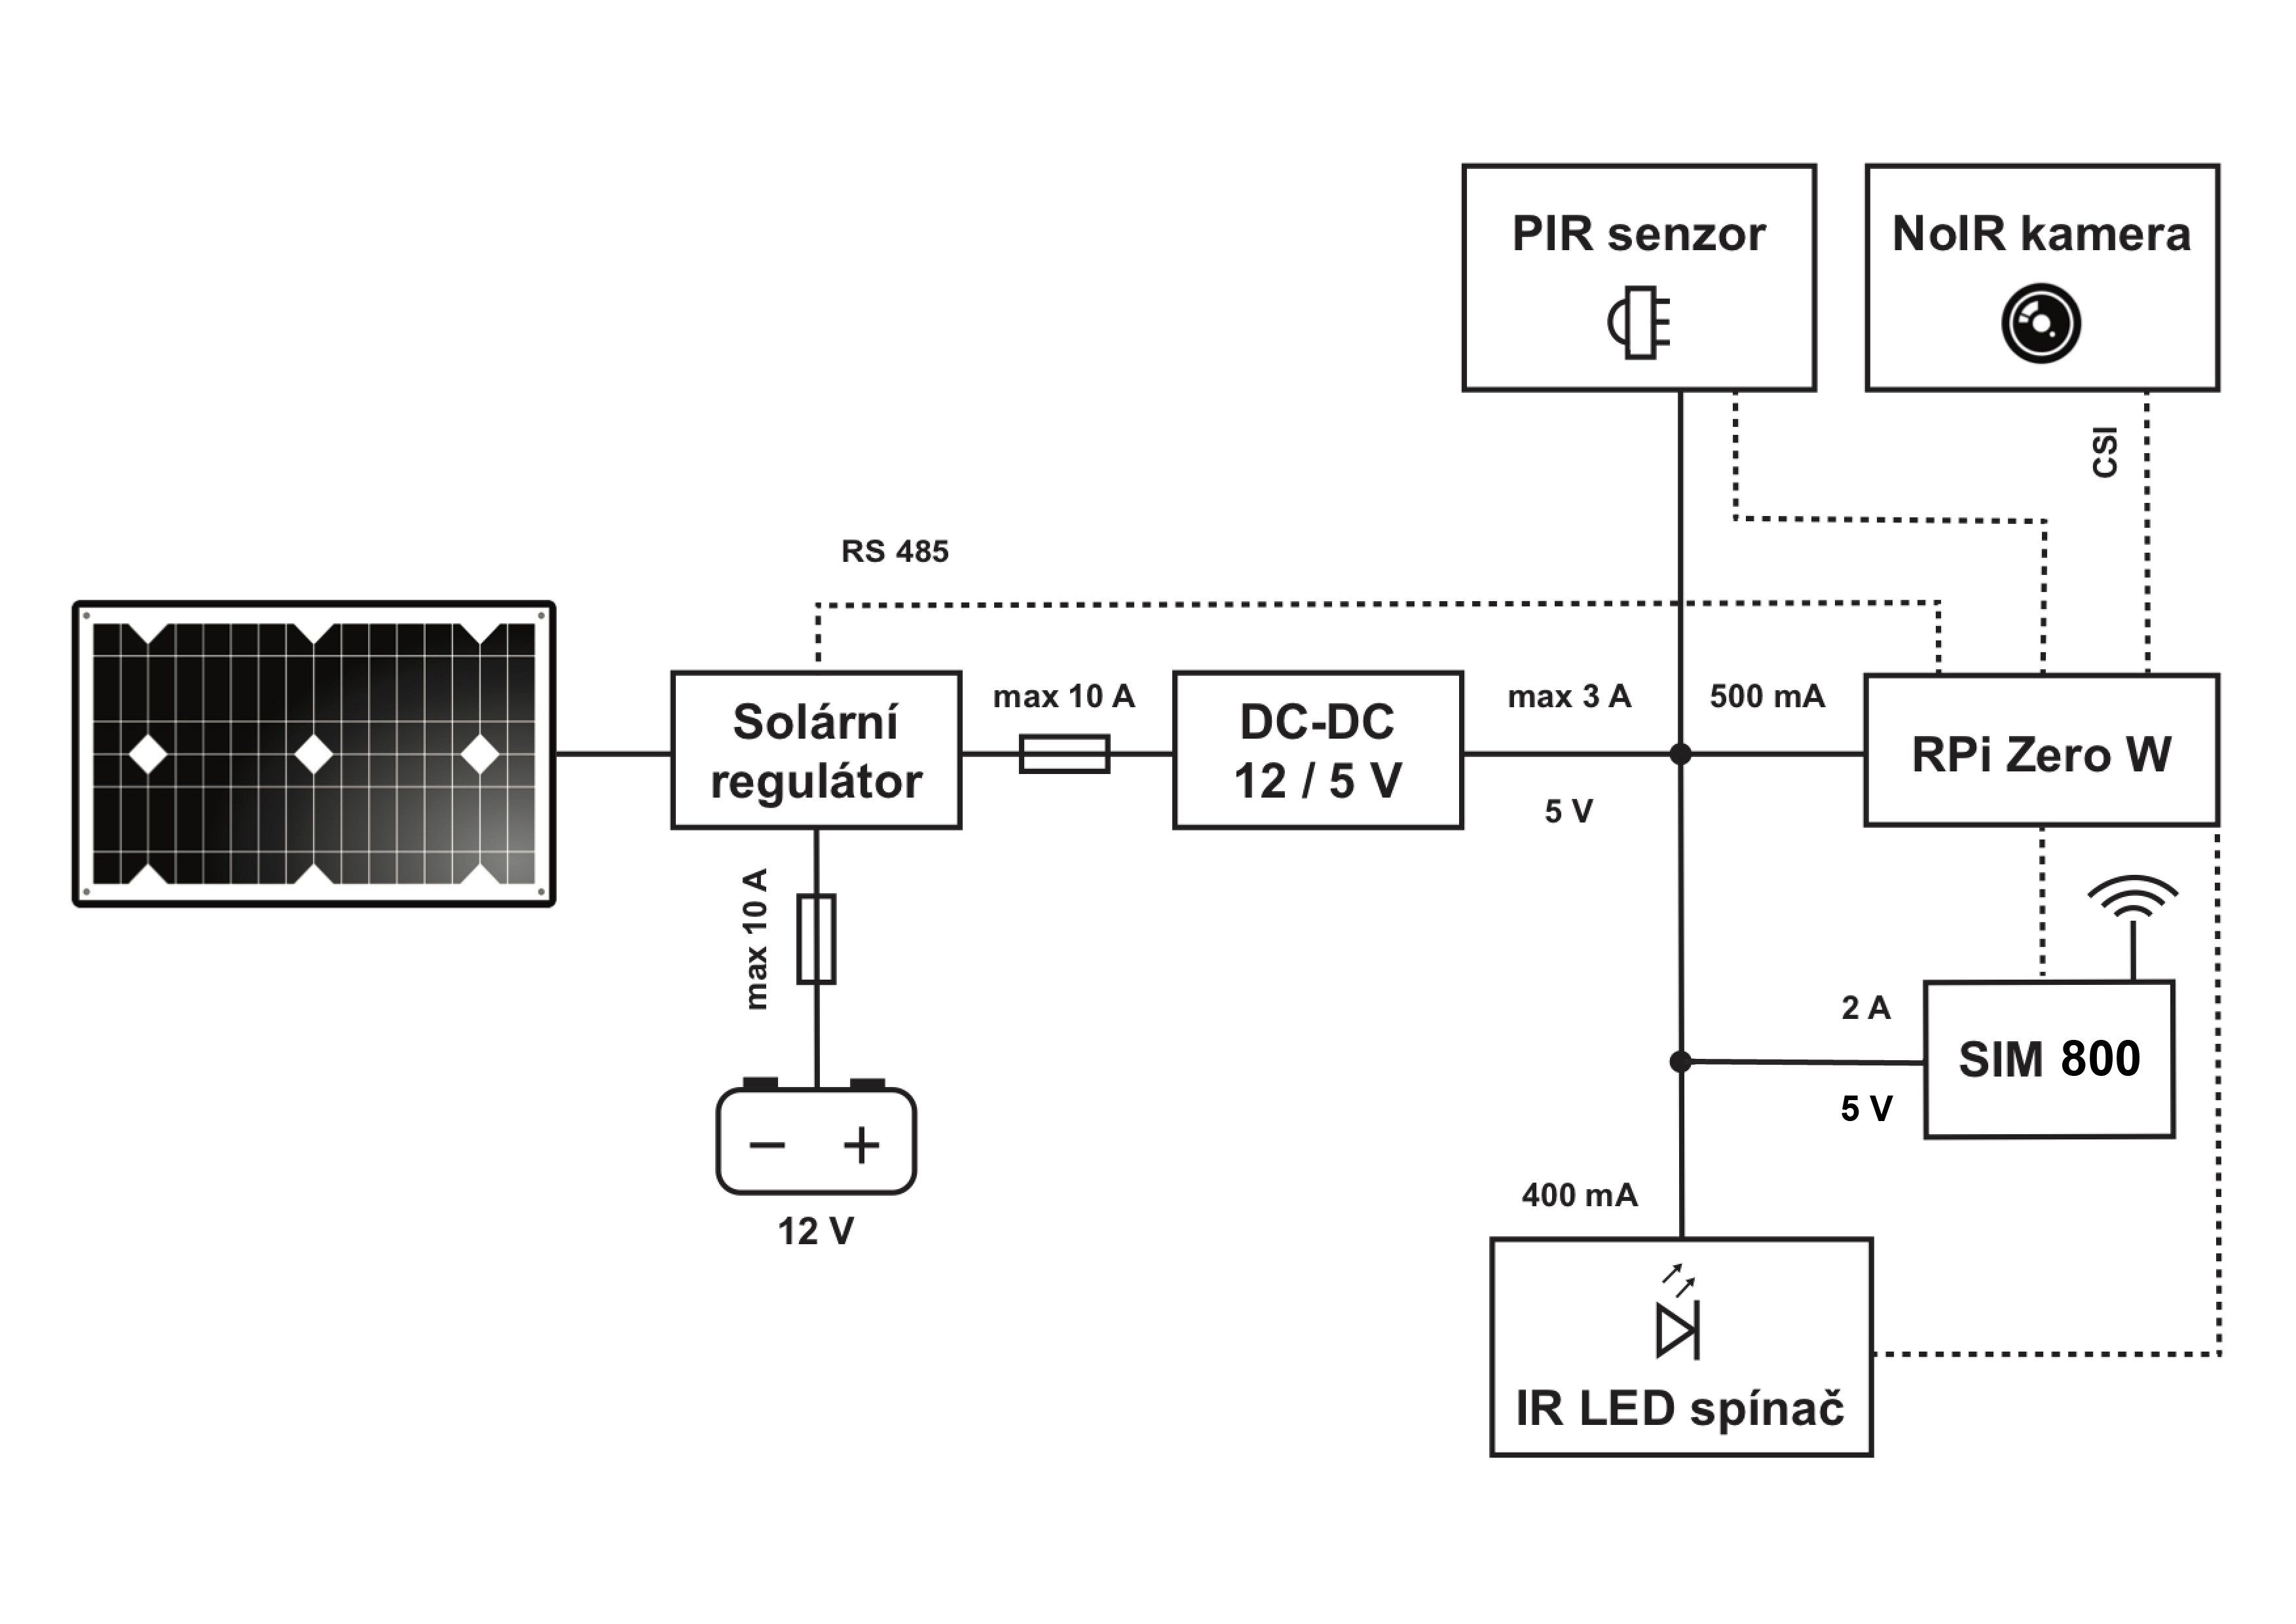
\includegraphics[scale=0.6, angle=90]{obrazky/blokove-schema-nove.png}
  \end{center}
  \caption{Blokové schéma návrhu zařízení}
\end{figure}

\clearpage

\section{Seznam a cena komponent}

\begin{table}[h]
\centering
\caption{Seznam komponent}
\label{komponenty}
\begin{tabular}{|l|l|l|}
\hline
\textbf{Jméno komponenty}                          & \textbf{Cena včetně DPH} \\ \hline
Raspberry Pi Zero W                                & 313 Kč (rpishop.cz)      \\ \hline
Raspberry Pi NoIR Camera Board V2                  & 858 Kč (rpishop.cz)      \\ \hline
SanDisk microSD karta 16 GB class 10                & 229 Kč (czc.cz)          \\ \hline
GSM/GPRS modul SIM800                              & 250 Kč                  \\ \hline
PIR modul HC-SR501                                 & 110 Kč (gme.cz)          \\ \hline
Výkonová IR LED dioda GT-P04IR4101                 & 45 Kč (gme.cz)           \\ \hline
Akumulátor Westinghouse WA12200                    & 1290 Kč (gme.cz)         \\ \hline
Solární panel WS-30/12V                            & 1990 Kč (gme.cz)         \\ \hline
Solární regulátor Epsolar LS1024B                  & 739 Kč (gme.cz)          \\ \hline
Převodník USB na RS-485                            & 240 Kč (rpishop.cz)        \\ \hline
DC/DC měnič 12V/5V CPT                             & 157 Kč                   \\ \hline
ULN20003A                                     & 10 Kč (gme.cz)           \\ \hline
Rezistor 22k                                       & 2,60 Kč (gme.cz)         \\ \hline
Drátový rezistor RD 12R 5W                         & 5,30 Kč (gme.cz)         \\ \hline
\end{tabular}
\end{table}

Cena komponent je platná k prosinci 2017.
